%=====================================================
% Template Laporan Tugas Akhir STTN-BATAN Yogyakarta
% Created and Arranged by :
% Abdurrohman Ibnul Mufadlol - 031700012
% email : ibnulmufadlol@gmail.com
% Created at : 2021
%=====================================================
%documentclass
\documentclass[a4paper,12pt,openright,oneside]{book}
% Load konfigurasi LaTeX untuk tipe laporan laporan tugas akhir
\usepackage{tugasakhir-sttn}
% package untuk include file pdf
\usepackage{pdfpages}
% package untuk membedakan configurasi halaman selanjutnya. contoh ada di sampul
\usepackage{afterpage}
%lokasi penyimpanan gambar
\graphicspath{{image/}}

% Daftar pemenggalan suku kata dan istilah dalam LaTeX atau biasa disebut pemenggalan kata
%\include{hype.indonesia}
% Daftar istilah yang mungkin perlu ditandai 
%\input{istilah}

% Awal bagian penulisan laporan
\begin{document}
	%
	% Sampul Laporan
	\begin{titlepage}
	%pagecolor{red} >> elmek pagecolor{yellow} >> elins
	\pagecolor{red}\afterpage{\nopagecolor}
	\thispagestyle{empty}
	\begingroup
	\begin{center}
		\singlespacing
		\textbf{TUGAS AKHIR}\\
		\fontsize{14pt}{1.5em}\selectfont
		\textbf{JUDUL TUGAS AKHIR UNTUK DIV STTN}\\[2cm]
		\fontsize{12pt}{1em}\selectfont
		Diajukan sebagai salah satu syarat untuk memperoleh gelar Sarjana Terapan Teknik\\[2cm]
		\fontsize{12pt}{1em}\selectfont
		\textbf{PROGRAM STUDI (...)}\\
		\textbf{JURUSAN TEKNOFISIKA NUKLIR}\\[2cm]
		
		\begin{figure}[h]
			\centering
			
\includegraphics[height=5cm]{sttn-bw-nobg}
		\end{figure}
		\vspace{2cm}
		
		Disusun oleh\\
		\textbf{NAMA MAHASISWA\\NIM}\\[2cm]
		
		\textbf{SEKOLAH TINGGI TEKNOLOGI NUKLIR\\BADAN TENAGA NUKLIR NASIONAL\\YOGYAKARTA\\2021}
	\end{center}
	\endgroup
\end{titlepage}
	%
	%
	% Gunakan penomeran romawi
	\pagenumbering{roman}
	% load halaman judul dalam
	\begin{titlepage}
	\thispagestyle{plain}
	\begingroup
	\begin{center}
		\singlespacing
		\textbf{TUGAS AKHIR}\\
		\fontsize{14pt}{1.5em}\selectfont
		\textbf{JUDUL TUGAS AKHIR UNTUK DIV STTN}\\[2cm]
		\fontsize{12pt}{1em}\selectfont
		Diajukan sebagai salah satu syarat untuk memperoleh gelar Sarjana Terapan Teknik\\[2cm]
		\fontsize{12pt}{1em}\selectfont
		\textbf{PROGRAM STUDI (...)}\\
		\textbf{JURUSAN TEKNOFISIKA NUKLIR}\\[2cm]
		
		\begin{figure}[h]
			\centering
			
\includegraphics[height=5cm]{sttn-bw}
		\end{figure}
		\vspace{2cm}
		
		Disusun oleh\\
		\textbf{NAMA MAHASISWA\\NIM}\\[2cm]
		
		\textbf{SEKOLAH TINGGI TEKNOLOGI NUKLIR\\BADAN TENAGA NUKLIR NASIONAL\\YOGYAKARTA\\2021}
	\end{center}
	\endgroup
\end{titlepage}
	\begin{titlepage}
	\thispagestyle{plain}
	\begingroup
	\begin{center}
		\singlespacing
		\textbf{FINAL PROJECT}\\
		\fontsize{14pt}{1.5em}\selectfont
		\textbf{TITLE OF FINAL PROJECT}\\[2cm]
		\fontsize{12pt}{1em}\selectfont
		Proposed as one of the requirements to obtain a Bachelor of Applied Engineering degree\\[2cm]
		\fontsize{12pt}{1em}\selectfont
		\textbf{(...) STUDY PROGRAMS}\\
		\textbf{NUCLEAR TECHNOFFICIAL DEPARTMENT}\\[2cm]
		
		\begin{figure}[h]
			\centering
			
\includegraphics[height=5cm]{sttn-bw}
		\end{figure}
		\vspace{2cm}
		
		Arranged by\\
		\textbf{NAMA MAHASISWA\\NIM}\\[2cm]
		
		\textbf{POLYTECHNIC INSTITUTE OF NUCLEAR TECHNOLOGY\\NATIONAL NUCLEAR ENERGY AGENCY\\YOGYAKARTA\\2021}
	\end{center}
	\endgroup
\end{titlepage}

	% setelah bagian ini, halaman dihitung sebagai halaman ke 2
	\setcounter{page}{2}
	
	%
	% load halaman pengesahan
	\begin{center}
	\begin{singlespace}
		{\normalfont\bfseries TUGAS AKHIR}\par\nobreak
		\vspace{0.5cm}
		{\normalfont\bfseries\MakeUppercase{JUDUL TUGAS AKHIR}}\par\nobreak
		\vspace{0.5cm}
		Dipersiapkan dan disusun oleh \\
		\vspace{0.5cm}
		{\normalfont\bfseries NAMA MAHASISWA}\\
		{\normalfont\bfseries NIM}\\
		\vspace{0.5cm}
		Telah dipertahankan di depan Dewan Penguji\\
		Pada tanggal $\dots\dots$\\
		dan dinyatakan telah memenuhi syarat \vspace{.5cm}\\
		
		{\underline{\bfseries{Susunan Dewan Penguji}}}\\
		\vspace{.5cm}
		
		\begin{singlespace}
			\begin{tabular}{lp{0.5cm}l}
				Ketua Dewan Penguji && Anggota I  \vspace{1.5cm}\\
				
				
				\underline{\bfseries{NAMA KETUA PENGUJI}}&& \underline{\bfseries{NAMA ANGGOTA PENGUJI I}} \\
				NIP.  && NIP. \vspace{.5cm}\\
				
				Anggota II && Pembimbing  \vspace{1.5cm}\\
				
				
				\underline{\bfseries{NAMA ANGOTA PENGUJI II}}&& \underline{\bfseries{NAMA PEMBIMBING TA}} \\
				NIP.  && NIP. 
			\end{tabular}
		\end{singlespace}
		
		
		\vspace{0.5cm}
		Tugas akhir ini telah diterima sebagai salah satu persyaratan  \\untuk memperoleh gelar Sarjana Terapan Teknik \vspace{0.3cm}\\
		
		Tanggal : $\dots\dots$\\
		Ketua Jurusan Teknofisika Nuklir \\
		
		\vspace{1.25cm}
		\begin{singlespace}\underline{\bfseries{NAMA KAJUR TFN}} \\
			NIP. 
		\end{singlespace}
		
		\vspace{0.3cm}
		Mengetahui,\\
		Ketua Sekolah Tinggi Teknologi Nuklir-BATAN\\
		
		\vspace{1.25cm}
		\begin{singlespace}
			\underline{\bfseries{NAMA KETUA STTN}} \\
			NIP. 
		\end{singlespace}
	\end{singlespace}
\end{center}
	%
	% load halaman orisinalitas 
	\addChapter{PERNYATAAN}
	\chapter*{HALAMAN PERNYATAAN}

\noindent Yang bertanda tangan di bawah ini :

\begin{tabular}{lcl}
	Nama & : & .................................................\\
	NIM & : & .................................................\\
	Program Studi &	: & .................................................\\
	Judul Tugas Akhir &	: & \uppercase{tuliskan judul anda disini}\\
\end{tabular}

\singlespacing
\noindent Dengan ini saya menyatakan bahwa tugas akhir ini tidak mengandung karya yang pernah diajukan untuk memperoleh gelar kesarjanaan di suatu Perguruan Tinggi, dan sepanjang pengetahuan saya juga tidak mengandung karya atau pendapat yang pernah ditulis atau diterbitkan oleh orang lain, kecuali yang secara tertulis diacu dalam naskah ini dan disebutkan dalam daftar pustaka.\\[2cm]

\begin{flushright}
	Yogyakarta, 21 Februari 2021\\[2cm]
	\underline{Nama Mahasiswa}\\
	NIM
\end{flushright}
	%
	%
	\addChapter{PRAKATA}
	\chapter*{PRAKATA}

\doublespacing
Puji syukur ke hadirat Allah SWT yang telah melimpahkan rahmat dan barokahnya sehingga penulis dapat menyelesaikan tugas akhir dengan judul \textbf{XXXXX}. Laporan tugas akhir ini disusun untuk memenuhi salah satu syarat dalam memperoleh gelar Sarjana Terapan Teknik (S.Tr.T) pada Program Studi DIV Teknofisika Nuklir Sekolah Tinggi Teknologi Nuklir BATAN.

Dalam melakukan penelitian dan penyusunan laporan tugas akhir ini penulis telah mendapatkan banyak dukungan dan bantuan dari berbagai pihak. Penulis mengucapkan terima kasih yang tak terhingga kepada:

\onehalfspacing
\begin{enumerate}
	\item Alloh SWT yang telah memberikan nikmat, rahmat dan hidayah serta inayahNya.
	\item Nama orang tua dan orang yang berperan dalam hidup saudara yang selalu mendoakan dan mendukung aku dalam menyelesaikan program studi elektronika intrumentasi/elektro mekanika diploma IV STTN-BATAN.
	\item Nama pembimbing utama selaku dosen pembimbing utama, dan nama pembimbing pendamping selaku dosen pembimbing pendamping, yang telah dengan penuh kesabaran dan ketulusan memberikan ilmu dan bimbingan terbaik kepada penulis. 
	\item Nama Ketua STTN-BATAN selaku Ketua STNN-BATAN dan Nama Ketua Jurusan Teknofisika Nuklir selaku Ketua Jurusan Teknofisika Nuklir yang memberikan izin kepada penulis untuk belajar.
	\item Para Dosen STTN-BATAN yang telah memberikan bekal ilmu kepada penulis.
	\item Para Karyawan/wati STTN-BATAN yang telah membantu penulis dalam proses belajar.
	\item Semua yang ingin disebutkan
	\item Teman-teman, kolega, dan keluarga besar penulis yang namanya belum tercantum di atas. Dukungan kalian adalah hal luar biasa yang sangat penulis syukuri.
\end{enumerate}

\doublespacing
Penulis menyadari sepenuhnya bahwa laporan tugas akhir ini masih jauh dari sempurna, untuk itu semua jenis saran, kritik dan masukan yang bersifat membangun sangat penulis harapkan. Akhir kata, semoga tulisan ini dapat memberikan manfaat dan memberikan wawasan tambahan bagi para pembaca dan khususnya bagi penulis sendiri.

\begin{flushright}
	Yogyakarta, 21 Februari 2021\\[1cm]
	Nama Mahasiswa
\end{flushright}
	%
	%
	%\addChapter{LEMBAR PERSETUJUAN PUBLIKASI ILMIAH}
	%\include{persetujuan_publikasi}
	%
	%menambahkan arti lambang dan singkatan
	\phantomsection
%	\addChapter{ARTI LAMBANG DAN SINGKATAN}
%	\printnomenclature[1.5cm]
	% load abstrak
	\addChapter{INTI SARI}
	\chapter*{INTI SARI}
\fontsize{14pt}{1.5em}\selectfont
\begin{center}
	\uppercase{\textbf{judul tugas akhir}}\\
\end{center}
\begin{tabular}{lcl}
	Nama & : & .................................................\\
	NIM & : & .................................................\\
	Pembimbing I &	: & .................................................\\
	Pembimbing II &	: & .................................................\\
\end{tabular}

\singlespacing
\noindent Disertasi ini membahas manifold \emph{upper half-plane} empat dimensi dan aplikasinya pada supergravitasi $N=2$ di lima dimensi. Manifold ini merupakan generalisasi dari metrik Joyce, yang merupakan salah satu referensi utama di riset ini. Solusi Pembahasan manifold \emph{upper half-plane} dimulai dengan analisis kestabilan dari potensial dan Hamiltonian. Hasil dari analisis tersebut menunjukkan bahwa potensial berkaitan dengan Hamiltonian saat potensialnya berada di titik kritis. Analisis dari kasus khusus metrik \emph{upper half-plane} untuk satu parameter menunjukkan bahwa metriknya tidak mungkin memenuhi syarat Einstein. Persamaan gerak dari aksi Riemann-Hilbert-nya dapat dilinearisasi sehingga memberikan solusi untuk aproksimasi orde pertama. Pembahasan di akhir disertasi mengarah kepada aplikasi metrik Joyce ke solusi \emph{domain wall} pada supergravitasi $N=2$ di lima dimensi. Dalam aplikasinya, solusi \emph{domain wall} akan mereduksi permasalahan empat dimensi menjadi permasalahan dua dimensi di ruang \emph{upper half-plane}. Syarat kestabilan dari persamaan aliran diperoleh dari matriks Hessian.

\noindent\textbf{Kata kunci:} \emph{domain wall}, Joyce, stabilitas, \emph{upper half-plane}
	\addChapter{ABSTRACT}
	\chapter*{ABSTRACT}
\fontsize{14pt}{1.5em}\selectfont
\begin{center}
	\uppercase{\textbf{title}}\\
\end{center}
\begin{tabular}{lcl}
	Name & : & .................................................\\
	Student Identity Number & : & .................................................\\
	Supervisor I &	: & .................................................\\
	Supervisor II &	: & .................................................\\
\end{tabular}

\singlespacing
\noindent The grinding process is a step in the metallographic test to produce a flat, smooth sample. The visual determination of samples makes the sample preparation time long enough. Therefore, a quality-based surface-test material is developed to measure the level of fineness of the sample. Samples grinding result is taken its image. The digital image of the sample will be processed using image processing which includes, preprocessing, feature extraction, and classification. The analyzed sample will be displayed in the form of a Graphical User Inteface (GUI) based decision that the sample can continue the process or repeat the preparation process. The results of this study are expected to help determine the level of surface quality of the materials in metallographic test preparation.

\noindent\textbf{Keywords:} Metallography, Digital image processing, GUI
	%
	% Daftar isi, gambar, dan tabel
	%
	\addChapter{DAFTAR ISI}
	\phantomsection %hack to make them clickable
	\tableofcontents
	\clearpage
	\addChapter{DAFTAR GAMBAR}
	\phantomsection %hack to make them clickable
	\listoffigures
	\clearpage
	\addChapter{DAFTAR TABEL}
	\phantomsection %hack to make them clickable
	\listoftables
	\clearpage
	
	%
	% Gunakan penomeran Arab (1, 2, 3, ...) setelah bagian ini.
	%
	\pagenumbering{arabic}
	
	%
	%
	%
	\chapter{\uppercase{Pendahuluan}}\label{pendahuluan}
\doublespacing
\section{Latar Belakang}
Dokumen ini adalah template Proposal Penelitian Tugas Akhir Jurusan Teknofisika Nuklir STTN-Batan. Bagian Pendahuluan berisi Latar Belakang, Rumusan Masalah, Batasan Penelitian, Keaslian Penelitian, Tujuan Penelitian dan Manfaat Penelitian. Uraikan artikel-artikel yang menjadi latar belakang penelitian ini dilakukan. Tuliskan apa yang sudah dilakukan oleh peneliti lain. Referensi menggunakan cara HAVARD. Kutipan diurutkan berdasar urut abfabet.  Tidak disarankan ada gambar di bagian pendahuluan. Jika sangat diperlukan adanya gambar, maka harus sesuai ketentuan. Lihat di bab selanjutnya mengenai gambar.

\section{Rumusan Masalah}
Perumusan masalah menjelaskan masalah yang ada sehingga penelitian perlu dilakukan. Diuraikan berdasarkan latar belakang penelitian yang sudah dijelaskan di sub sebelummnya. Perumusan masalah hanya berupa masalah, bukan apa yang dilakukan. Perumusan masalah biasanya bernada negatif yang perlu diselesaikan pada tujuan penelitian. Tidak ada sitasi. Bagian ini murni tulisan sendiri.

\section{Batasan Masalah}
Jelaskan apa yang akan dilakukan dan apa yang tidak akan dilakukan dalam penelitian. Batasan juga dapat menjelaskan batasan alat, bahan, ataupun data penelitian.

Pembatasan masalah dalam penelitian ini perlu dilakukan agar dalam pembahasannya lebih terarah dan sistematis.

\section{Keaslian Penelitian}
Jelaskan novelty atau kontribusi penelitian di sini. Uraikan dari latar belakang dengan lebih menonjolkan peran penelitian anda. Akan lebih banyak sitasi di sini dibandingkan di bagian latar belakang. Jika ada kekurangan peneliti lain, sehingga proposal penelitian ini penting, ungkapkan di bagian ini. Cara penulisan keaslian penelitian boleh dalam bentuk tabel, \textit{fish bone diagram} maupun narasi. Penulisan Nama-Tabel menggunakan tabular seperti contoh dibawah, sedangkan untuk mengacu nama tabel gunakan reference pada label seperti ini (Tabel \ref{tabel Al}). %\ref{nama_tabel}.

\begin{table}[!htb] \index{Hasil HVL}
	\begin{center}
		\caption[Contoh HVL]{Hasil Percobaan HVL Alumunium vs $^{60}$Co}
		\label{tabel Al}
		\begin{tabular}{ccccc}
			\hline
			Ketebalan (inch) & Cacahan rata-rata & N (cps) & N\textsubscript{0} (cps) & $\ln\left(\frac{N}{N_0}\right)$\\
			\hline
			0.125 & 358.67 & 11.15 & 15.02 & -0.2934\\
			0.08 & 356 & 11.06 & 15.02 & -0.3024\\
			0.02 & 413.33 & 12.98 & 15.02 & -0.1444\\
			\hline
		\end{tabular}
	\end{center}
\end{table}

\section{Tujuan Penelitian} \label{tujuan}
Judul bab atau subbab baru tidak boleh sendiri di bawah. Jika terpaksa sendirian di bawah, enter satu kali sehingga masuk halaman baru. 

Tujuan penelitian menerangkan apa yang ingin dicapai dari penelitian. Bagian ini adalah jawaban dari perumusan masalah yang diuraikan sebelumnya. Jika dimungkinkan, jelaskan ukuran keberhasilan dari penelitian yang akan dilakukan. Tujuan penelitian dapat lebih dari satu, namun tetap menjawab/menyelesaikan masalah. Jika tujuan penelitian lebih dari satu, tuliskan dengan bullet atau numbering.

\section{Manfaat Penelitian}
Jelaskan manfaat yang diperoleh jika penelitian berhasil. Jelaskan baik dari sisi ilmu pengetahuan maupun kemanfaatannya bagi masyarakat. Akan sangat baik jika ada manfaat bagi bangsa dan negara.
	\chapter{\uppercase{Dasar Teori}}\label{dasarteori}

\section{Tinjauan Pustaka}
Jelaskan paper-paper dan penelitian yang terkait dengan penelitian anda di sini. Sitasi mungkin akan lebih banyak lagi di sini. Penulisan Sitasi dapat dilihat pada dokumentasi tata cara penggunaan \LaTeX. Penelitian-penelitian pendukung yang lebih banyak sebaiknya diungkapkan untuk memperjelas arah penelitian anda.  Penjelasan mengenai novelty anda lebih banyak diuraikan lagi.

Uraikan novelty atau kontribusi penelitian dari keaslian penelitian dengan lebih detail di sini. Tonjolkan peran penelitian anda dengan menjelaskan penelitian yang sudah ada dengan gap penelitian yang akan diselesaikan. Akan lebih banyak sitasi. Jika ada kekurangan peneliti lain, sehingga proposal penelitian ini penting, ungkapkan di bagian ini dengan lebih detail.

\section{Topik Teori yang Dibutuhkan} \label{teori}
Pada subbab ini dibahas mengenai dasar teori yang dipakai serta justifikasinya untuk menyelesaikan penelitian. Sitasi dari berbagai sumber, termasuk buku, web dan sumber yang lain dimungkinkan. Tidak diperkenankan mengambil sumber yang tidak jelas asalnya, seperti blog pribadi dan/atau wiki. Dasar teori yang mendasari penelitian termasuk rumus-rumus, algoritma yang akan dikembangkan, gambar, struktur diagram, dan lain-lain diungkapkan di sini. Contoh penggunaan sitasi adalah sebagai berikut \citep{contohdafpus}. Penambahan daftar pustaka dapat dilakukan dalam file \code{DaftarPustaka.bib}.

\subsection{Subsection yang lebih kecil}
Penulisan proposal dimungkinkan untuk membentuk subbab- subbab yang lebih kecil, namun disarankan untuk tidak lebih dari tiga poin angka, sebagaimana dalam contoh ini. Sebagai gantinya, subbab yang lebih dari tiga poin menggunakan huruf besar dan cetak miring.

\subsubsection{Gambar dan Grafik} \label{gambar}
Setiap gambar maupun grafik harus diberi nomor dan diberi judul dengan perintah \code{\textbackslash caption\{nama\}}, sebagaimana terlihat dalam contoh Gambar \ref{contohgambar}. Setiap gambar harus ditunjuk di dalam narasi menggunakan perintah \code{\textbackslash ref\{nama\}} dan pemberian label dengan perintah \code{\textbackslash label\{nama\}}. Tidak hanya ditunjuk saja, namun gambar juga harus diterangkan makna gambar di dalam narasi.

Dalam contoh ini, Gambar \ref{contohgambar} menjelaskan tentang kurva HVL. Demikian seterusnya dijelaskan per bagian serta makna istilah-istilah di dalam gambar. Font di dalam gambar harus seragam dan harus dapat dibaca dengan jelas. 

Jika terdapat lebih dari satu gambar, maka antara gambar yang satu dengan yang lain harus senada. Maksud senada adalah jenis dan besar font sama atau tidak jauh berbeda. Demikian juga dengan penggunaan garis, kotak dan lain-lain, harus sama atau hampir sama.

\begin{figure}
	\centering
	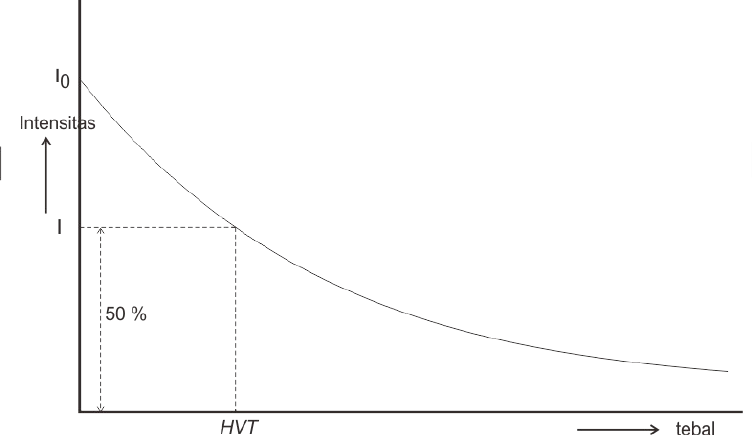
\includegraphics{kurva1}
	\caption{Kurva Intensitas Radiasi vs Tebal Bahan}
	\label{contohgambar}
\end{figure}

\subsubsection{Tabel}
Judul tabel diletakkan di atas dengan rata tengah (center). Tabel \ref{contohtabel} adalah contoh tabel. Font dan penampakan tabel disesuaikan agar tabel tampak bagus dan mudah dibaca. Spasi single. Tabel harus dirujuk di dalam narasi dengan perintah yang sama seperti bagian \ref{gambar}. Makna tabel, baik keterangan maupun nilainya harus dijelaskan. Disarankan letak tabel berada di bagian paling atas atau paling bawah halaman atau berada di akhir (sub) bab. Lakukan sitasi ketika sebuah tabel diambil dari referensi tertentu. 

\begin{table}[!htb]
	\begin{center}
		\caption[Contoh HVL]{Hasil Percobaan HVL Alumunium vs $^{60}$Co}
		\label{contohtabel}
		\begin{tabular}{ccccc}
			\hline
			Ketebalan (inch) & Cacahan rata-rata & N (cps) & N\textsubscript{0} (cps) & $\ln\left(\frac{N}{N_0}\right)$\\
			\hline
			0.125 & 358.67 & 11.15 & 15.02 & -0.2934\\
			0.08 & 356 & 11.06 & 15.02 & -0.3024\\
			0.02 & 413.33 & 12.98 & 15.02 & -0.1444\\
			\hline
		\end{tabular}
	\end{center}
\end{table}

\subsubsection{Rumus dan Persamaan} \label{rumus}
Rumus dan persamaan dituliskan pada Bab 2. Cara penulisan persamaan menggunakan \code{equation} dan bantuan \code{tabular} seperti ditunjukkan pada Persamaan \ref{contohpersamaan}. Seluruh rumus atau persamaan yang dituliskan harus diacu pada paragraph dan disarankan untuk digunakan pada Bab 3 maupun Bab 4.

\begin{equation}\label{contohpersamaan}
	I=I_0.e^{-\mu.x}
\end{equation}

dengan

\begin{tabular}{lcl} 
	$I_0$ &	= & Intensitas paparan radiasi yang datang (mR/jam)\\
	$I$ &	= & Intensitas paparan radiasi yang diteruskan (mR/jam)\\
	$\mu$ &	= & Koefisienn serap linier bahan pada energi tertentu (mm\textsuperscript{-1})\\
	$x$ &	= & Tebal bahan (mm)\\
\end{tabular}

\subsection{Kesalahan penulisan yang sering terjadi}
Disarankan menggunakan kalimat yang lugas dan jelas. Hindari penggunaan anak kalimat yang berlebihan. Jika terpaksa ada anak kalimat, usahakan hanya satu anak saja. Penggunaan banyak anak kalimat atau bahkan beranak cucu akan membingungkan pembaca dalam menangkap maksud kalimat. Gunakan Bahasa Indonesia dengan baik dan benar.

Gunakan tata bahasa secara benar. Pastikan mana yang benar, di mana atau dimana, ke dua atau kedua, dan lain-lain. 

\section{Hipotesis}
Tuliskan hipotesis/pertanyaan penelitian anda berdasarkan tujuan penelitian yang ingin dicapai.
	\chapter{\uppercase{metode penelitian}} \label{metode_penelitian}
Metode penelitian membahas segala sesuatu yang dilakukan untuk mencapai tujuan. Bab ini minimal berisi alat-alat yang digunakan, baik \textit{hardware} maupun \textit{software}, bahan yang dipakai, dan langkah-langkah penelitian.

\section{Tempat dan Waktu}
Tuliskan tempat dan waktu pelaksanaan penelitian saudara.

\section{Alat Penelitian}
Sebutkan alat-alat yang dipakai beserta spesifikasinya. Jika diperlukan disertai dengan kegunaannya. Alat yang dipakai dalam penelitian ini adalah:
\begin{enumerate}
	\item Komputer 2 buah.\\
	Komputer ini satu digunakan sebagai client dan satu sebagai server. dan seterusnya dan seterusnya.
	\item Laptop
	\item MATLAB (semua alat di muka adalah contoh)
\end{enumerate}

\section{Bahan Penelitian}
Sebutkan bahan penelitian yang dipakai. Anda harus dapat membedakan antara alat dan bahan. Alat adalah perangkat untuk mengolah bahan, sedangkan bahan adalah yang diolah. Data penelitian dapat dimasukkan sebagai bahan, atau dapat dibuat subbab tersendiri. Sebutkan ada berapa data, dan diambil dari mana dan/atau bagaimana cara memperolehnya.

\section{Rencana Penelitian}
Sebutkan langkah-langkah penelitian yang akan ditempuh untuk meraih tujuan penelitian yang ingin dicapai (lihat Tujuan di Bab 1. Ungkapkan dalam bentuk gambar flowchart. Jelaskan maksud flowchart anda. Gambar \ref{langkahpenelitian} adalah contoh langkah-langkah penelitian.
	\begin{figure}
		\centering
		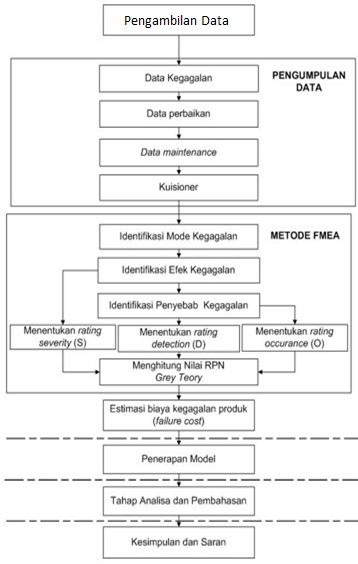
\includegraphics{langkahpenelitian}
		\caption{Langkah Penelitian}
		\label{langkahpenelitian}
	\end{figure}
	
	Tidak perlu menyertakan studi literatur di dalam langkah penelitian. Studi literatur sudah jelas dilakukan pada setiap penelitian apapun. Jelaskan masing-masing tahapan pada Gambar \ref{langkahpenelitian} yang dilakukan. Jelaskan tahapan-tahapan ini dalam subsection yang berurutan.
	
	Selain langkah penelitian, gambar sistem yang dirancang perlu digambarkan. Gambar sistem harus disertakan ketika penelitian mengandung unsur perancangan sistem. Gambar \ref{perancagansistem} adalah contoh gambar sistem.
	\begin{figure}
		\centering
		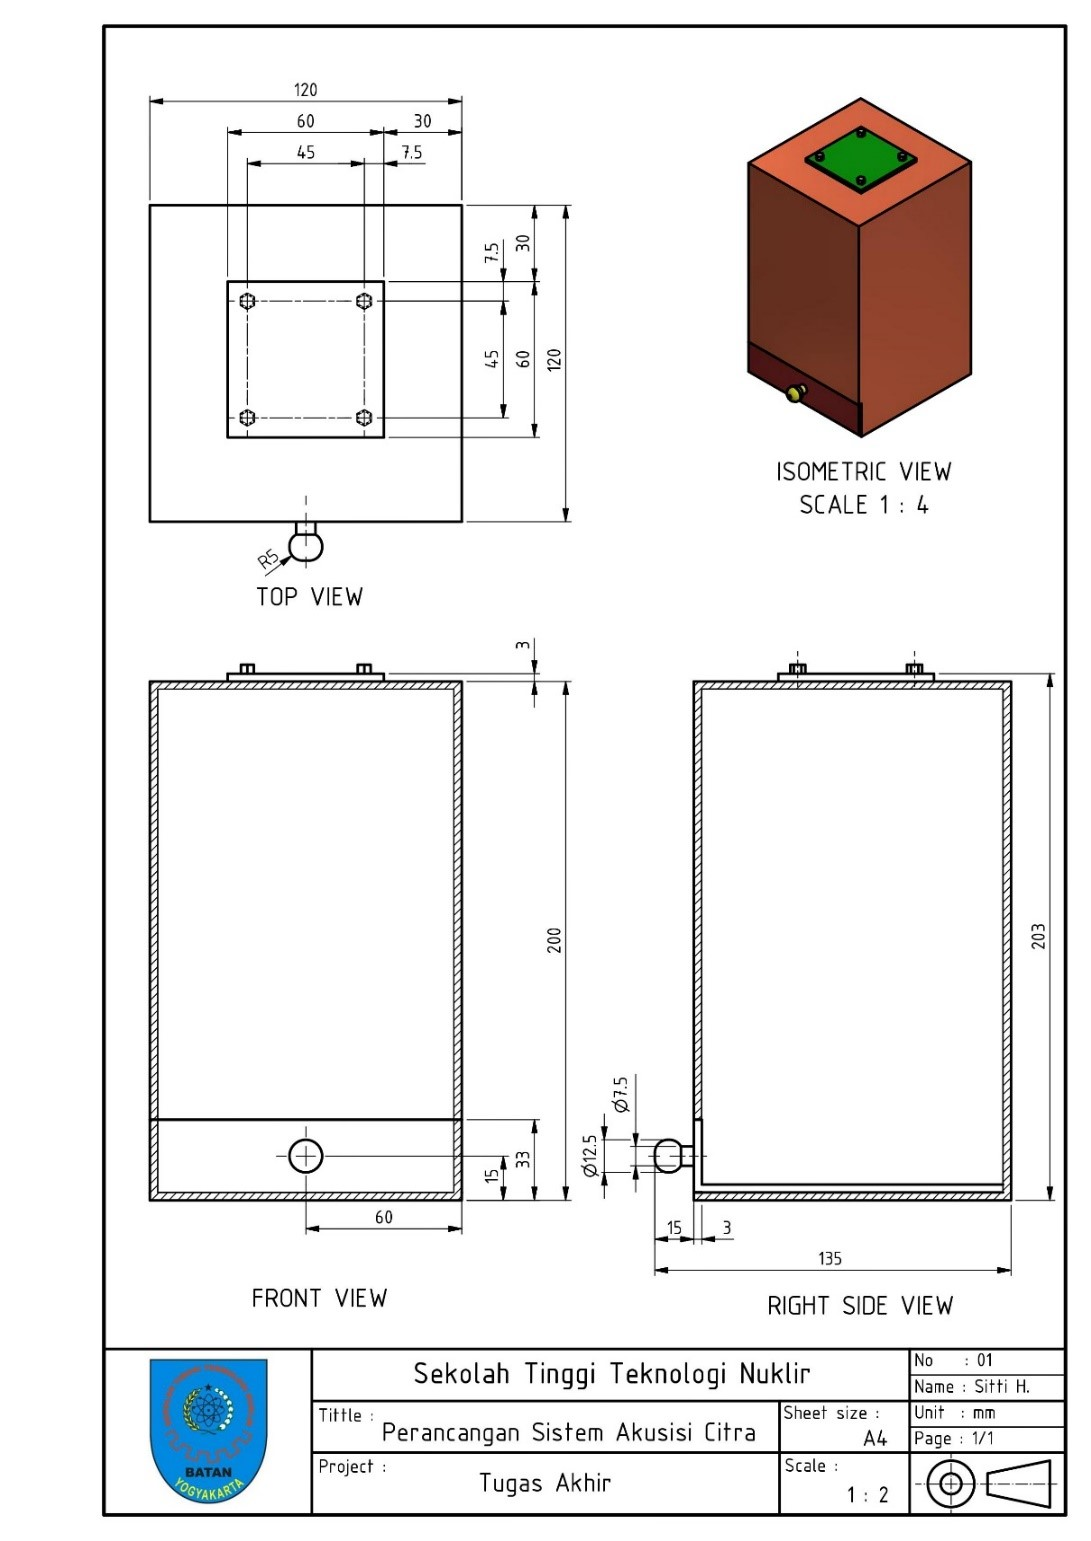
\includegraphics{perancangan_sistem}
		\caption{Perancangan Sistem}
		\label{perancagansistem}
	\end{figure}
	
	Gunakan simbol diagram yang tepat. Jelaskan makna Gambar \ref{perancagansistem} secara keseluruhan, serta jelaskan makna masing-masing bagiannya
	
	Ungkapkan hal-hal lain dalam penelitian jika dirasakan perlu. Hal-hal yang perlu diungkapkan mungkin saja berupa kesulitan-kesulitan, keterbatasan alat, kesulitan pengambilan data, dan lain-lain. Sebutkan bagaimana cara mengatasi atau skenario ketika gagal karena kesulitan/keterbatasan tersebut. Hal lain ini dapat juga berupa modal penelitian sebelumnya yang berhasil.
	
	Pada Bab ini selain dijelaskan cara perancangan dan pembuatan juga harus dijelaskan cara analisis (metode pengujian) yang akan dilakukan.
	
	\section{Metode Analisis}
	Tuliskan langkah-langkah dalam melakukan analisis. Langkah-langkah ini harus dilandasi di section 2.2. \ref{rumus}
	\chapter{\uppercase{hasil dan pembahasan}} \label{bab4}
Tuliskan hasil-hasil penelitian berdasar langkah-langkah yang disebutkan di Bab III (Metode). Kemudian lakukan analisis hasil berdasar langkah-langkah yang ditunjukkan di sub-bab 3.4. Dalam melakukan analisis jangan sampai menyimpang dari Sub-bab 2.2 (Landasan Teori) dan Sub-bab 1.4 (Tujuan Penelitian)

%perbaikan pada \ref{}untuk beda file
		\chapter{\uppercase{kesimpulan dan saran}} \label{bab5}
\section{Kesimpulan} \label{kesimpulan}
Pada sub-bab ini dituliskan kesimpulan hasil penelitian atau kesimpulan TA. Kesimpulan harus ditulis berdasarkan hasil penelitian, pembahasan, dan temuan yang telah ditulis pada bab sebelumnya yang tentu saja disesuaikan dengan tujuan penelitian atau TA. Jangan menyimpulkan sesuatu yang tidak ada di dalam pembahasan yang telah dibuat. Kesimpulan dibuat dengan singkat dan jelas dengan urutan yang sebisa mungkin sesuai dengan tujuan penelitian (tertulis pada sub-bab tujuan penelitian).

Kesimpulan merupakan intisari dari pembahasan yang bersifat lebih general. Kesimpulan harus disesuaikan dengan hipotesis dan atau tujuan penelitian, dan juga harus dibuktikan di Bab IV (Hasil dan Pembahasan).

Kesimpulan boleh diberi nomor atau boleh juga tidak menggunakan nomor. Jika menggunakan nomor maka sesuai dengan template ini.

Jika tidak menggunakan nomor maka gunakan alenia-alenia sebagaimana ketentuan paragraph penulisan tesis seperti bab-bab sebelumnya.

\section{Saran} \label{saran}
Pada sub-bab ini dituliskan saran yang diusulkan oleh penulis. Dalam hal ini ada dua jenis saran:
\begin{enumerate}
	\item Saran untuk penelitian selanjutnya / kajian lanjutan. Saran jenis ini diberikan pada TA yang bersifat penelitian dan modelling. Saran ini berisi berbagai hal yang belum dilakukan, atau belum selesai dilakukan, atau berbagai hal yang merupakan lanjutan penelitian yang telah dilakukan dalam TA ini. Saran yang dibuat harus berdasarkan pembahasan serta kesimpulan yang telah dibuat. Jangan menyarankan sesuatu yang berada di luar jangkauan pembahasan dan kesimpulan yang dibuat.
	\item Saran terhadap perbaikan sistem yang dibahas dalam TA / practical implication. Saran jenis ini diberikan pada TA yang bersifat studi kasus. Saran ini berisi berbagai hal yang harus dilakukan untuk perbaikan sistem yang telah dibahas dalam sub-bab pembahasan dan kesimpulan. Saran yang diberikan hasus masuk akal dan mungkin untuk dilakukan / diaplikasikan. Saran ini tentunya berdasarkan temuan yang diperoleh dalam pembahasan dan disimpul-kan dalam sub-bab kesimpulan. Jangan memberikan saran yang berbeda / menyimpang dengan apa yang dibahas dan disimpulkan pada sub-bab pembahasan dan kesimpulan.
\end{enumerate}
	
	%
	% Daftar Pustaka
	\makeatletter
	\let\@chapter\orig@chapter
	\makeatother
	
	%Bagian Referensi
	\setstretch{1}
	\bibliography{DaftarPustaka} \addChapter{DAFTAR PUSTAKA} %daftar pustaka dapat diedit dengan teks editor biasa, contoh vscode, notepad++
	
	%Bagian Lampiran
	\setstretch{1.5}
	\cleardoublepage
	\appendix
	\addChapter{LAMPIRAN}
	%\topskip0pt
	\vspace*{\fill}
	\begin{center}
		\textbf{\large LAMPIRAN}
	\end{center}
	\vspace*{\fill}
	
	%Redefine text before appendix
	\makeatletter
	\let\orig@chapter\@chapter
	\def\@chapter[#1]#2{\ifnum \c@secnumdepth >\m@ne
		\if@mainmatter
		\refstepcounter{chapter}%
		\typeout{\@chapapp\space\thechapter.}%
		\addcontentsline{toc}{chapter}%
		{Lampiran~\protect\numberline{\thechapter}#1}%
		\else
		\addcontentsline{toc}{chapter}{#1}%
		\fi
		\else
		\addcontentsline{toc}{chapter}{#1}%
		\fi
		\chaptermark{#1}%
		\addtocontents{lof}{\protect\addvspace{10\p@}}%
		\addtocontents{lot}{\protect\addvspace{10\p@}}%
		\if@twocolumn
		\@topnewpage[\@makechapterhead{#2}]%
		\else
		\@makechapterhead{#2}%
		\@afterheading
		\fi}
	\makeatother
	
%	Include file lampiran
%	\include{LAMPIRAN1} >> untuk lampiran dalam bentuk .tex file
%	\includepdf{namafilepdf} >> untuk lampiran dalam bentuk .pdf
	%index
%	\backmatter
%	\phantomsection
%	\addChapter{INDEKS}
%	\printindex

	
\end{document}